\documentclass[11pt]{article}

\usepackage[a4paper,margin=2.1cm]{geometry}
\usepackage{amsmath,amssymb}
\usepackage{graphicx}
\usepackage{booktabs}
\usepackage{multirow}
\usepackage{tikz}
\usetikzlibrary{arrows.meta,positioning,shapes.geometric,calc,fit,backgrounds}
\usepackage{pgfplots}
\pgfplotsset{compat=1.18}
\usepackage{hyperref}
\usepackage{microtype}
\usepackage{caption}
\usepackage{framed}
\captionsetup{font=small,labelfont=bf}
\usepackage{xcolor}

\definecolor{goodg}{RGB}{34,139,34}
\definecolor{badr}{RGB}{200,40,40}
\definecolor{quboc}{RGB}{214,39,40}
\definecolor{cardbg}{RGB}{245,247,250}
\definecolor{cardline}{RGB}{180,190,205}
\definecolor{goldbg}{RGB}{255,250,235}
\definecolor{goldline}{RGB}{210,180,90}

\newenvironment{card}{%
  \def\FrameCommand{\fboxsep=8pt\fcolorbox{cardline}{cardbg}}%
  \MakeFramed{\advance\hsize-\width\FrameRestore}\noindent}{\endMakeFramed}
\newenvironment{goldcard}{%
  \def\FrameCommand{\fboxsep=8pt\fcolorbox{goldline}{goldbg}}%
  \MakeFramed{\advance\hsize-\width\FrameRestore}\noindent}{\endMakeFramed}

\newcommand{\good}[1]{\textcolor{goodg}{\textbf{#1}}}
\newcommand{\bad}[1]{\textcolor{badr}{\textbf{#1}}}
\newcommand{\key}[1]{\textcolor{quboc}{\textbf{#1}}}
\newcommand{\code}[1]{\texttt{#1}}

\title{\textbf{The Rover Fleet Project: A Guided Tour}\\[4pt]
\large Constrained graph pruning + trust-aware GNN task assignment,\\
explained simply --- and then in full detail, with the real numbers}
\author{Companion document to the paper \emph{Constrained Edge Pruning and
Trust-Aware GNN Inference for Task Allocation in Dynamic Rover Networks}}
\date{September 2026 \,\textbullet\, all numbers from the repository's own
experiment logs}

\begin{document}
\maketitle

\begin{goldcard}
\textbf{How to read this document.} Every number in it is real: it comes from
the experiment logs committed next to the code
(\code{benchmark.jsonl}, \code{benchmark\_bf0.75.jsonl},
\code{sweep\_*.jsonl}, \code{worked\_example.json}) or from the paper's
regression harness. Nothing is invented, rounded in our favor, or cherry
picked --- the embarrassing numbers are in here too, because they are the
interesting ones. Each section has a \emph{simple} version (what to say in
the meeting) and a \emph{detail} version (what to say when someone digs in).
\end{goldcard}

\tableofcontents
\vspace{4mm}

% ======================================================================
\section{The problem in one picture}
% ======================================================================

\begin{card}
\textbf{Simple version.} A team of rovers explores an area with no
infrastructure. They talk to each other over short-range radio links that
appear and disappear as they move. Every cycle, three things must happen:
\textbf{(1)} decide which radio links are worth using,
\textbf{(2)} decide which rover does which task, and
\textbf{(3)} actually deliver the results back to base --- over the links
you kept. Bad link choices silently break \emph{(3)}; bad task choices waste
the fleet. This project builds a system that makes both decisions
automatically, under hard rules (``no rover talks to more than $D$
others'', ``don't spend more compute than the budget''), and --- unusually
--- \emph{measures itself honestly} to find out whether the fancy
optimization is actually worth it.
\end{card}

\begin{figure}[h]
\centering
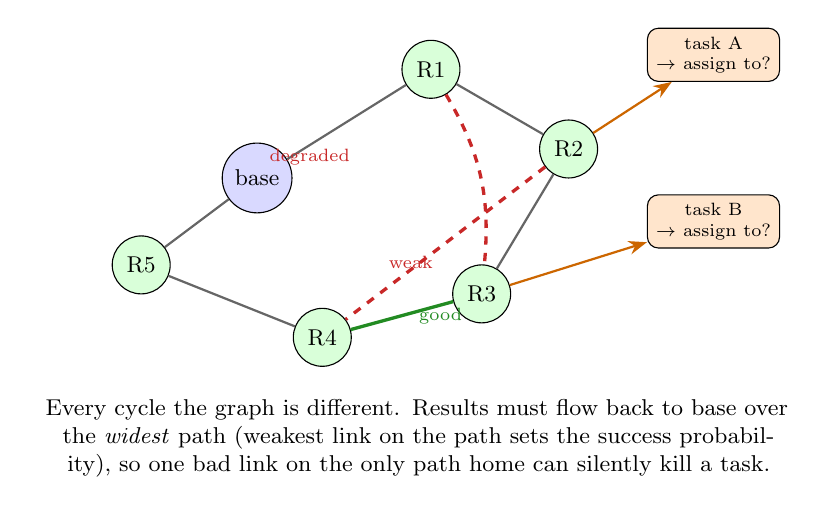
\begin{tikzpicture}[scale=0.92, every node/.style={transform shape}]
  % rovers
  \node[draw, circle, fill=blue!15, minimum size=9mm] (base) at (0,0) {\small base};
  \node[draw, circle, fill=green!15, minimum size=8mm] (r1) at (2.4,1.5) {\small R1};
  \node[draw, circle, fill=green!15, minimum size=8mm] (r2) at (4.3,0.4) {\small R2};
  \node[draw, circle, fill=green!15, minimum size=8mm] (r3) at (3.1,-1.6) {\small R3};
  \node[draw, circle, fill=green!15, minimum size=8mm] (r4) at (0.9,-2.2) {\small R4};
  \node[draw, circle, fill=green!15, minimum size=8mm] (r5) at (-1.6,-1.2) {\small R5};
  % links
  \draw[thick, black!60] (base) -- (r1);
  \draw[thick, black!60] (r1) -- (r2);
  \draw[thick, black!60] (r2) -- (r3);
  \draw[very thick, goodg] (r3) -- (r4) node[midway, right=1mm, font=\scriptsize, text=goodg] {good};
  \draw[thick, black!60] (r4) -- (r5);
  \draw[thick, black!60] (r5) -- (base);
  \draw[very thick, badr, dashed] (r1) to[bend left=18] (r3) node[midway, above right=0.5mm, font=\scriptsize, text=badr] {degraded};
  \draw[very thick, badr, dashed] (r2) -- (r4) node[midway, below left=0.5mm, font=\scriptsize, text=badr] {weak};
  % tasks
  \node[draw, rounded corners, fill=orange!20, font=\scriptsize, align=center] (t1) at (6.3,1.7) {task A\\ $\rightarrow$ assign to?};
  \node[draw, rounded corners, fill=orange!20, font=\scriptsize, align=center] (t2) at (6.3,-0.6) {task B\\ $\rightarrow$ assign to?};
  \draw[-Stealth, thick, orange!80!black] (r2) -- (t1);
  \draw[-Stealth, thick, orange!80!black] (r3) -- (t2);
  \node[font=\small, align=center, text width=10.5cm] at (2.2,-3.6)
    {Every cycle the graph is different. Results must flow back to base over
     the \emph{widest} path (weakest link on the path sets the success
     probability), so one bad link on the only path home can silently
     kill a task.};
\end{tikzpicture}
\caption{The world: 10 rovers (here 5 for legibility), links that come and
go, tasks that must be assigned, and a base that must receive the results.}
\end{figure}

\begin{card}
\textbf{Detail version.} The simulator (10 rovers, 20-cycle episodes,
3 tasks per cycle, drifting per-rover reliability) generates a dynamic
candidate graph each cycle. Each candidate link carries six normalized
features measured online: \emph{trust} (an exponentially-weighted estimate of
that rover's past delivery behavior), \emph{link quality}, \emph{battery},
\emph{proximity}, \emph{freshness} (how recent the observation is), and
\emph{task criticality}, plus a \emph{processing cost}. Two decisions are
made per cycle:

\begin{enumerate}
\item \textbf{Pruning} --- choose a subset of links to keep, subject to hard
constraints: per-node degree caps, a global processing budget, and exact
connectivity of the mission-critical node set to the base. This is
formulated as a QUBO (quadratic unconstrained binary optimization) and
solved in the cloud tier.
\item \textbf{Assignment} --- give each task to the rover with the best
expected outcome, scored by a trust-aware graph neural network running on
the pruned graph, in the fog tier.
\end{enumerate}

Mission success is \emph{causally} tied to pruning: a task's result is
delivered with probability equal to the widest-path bottleneck (the weakest
link on the best path) from the assigned rover to base \emph{on the kept
graph}. Prune badly and delivery fails --- the metric cannot be gamed.
\end{card}

% ======================================================================
\section{The pipeline, start to finish}
% ======================================================================

\begin{figure}[h]
\centering
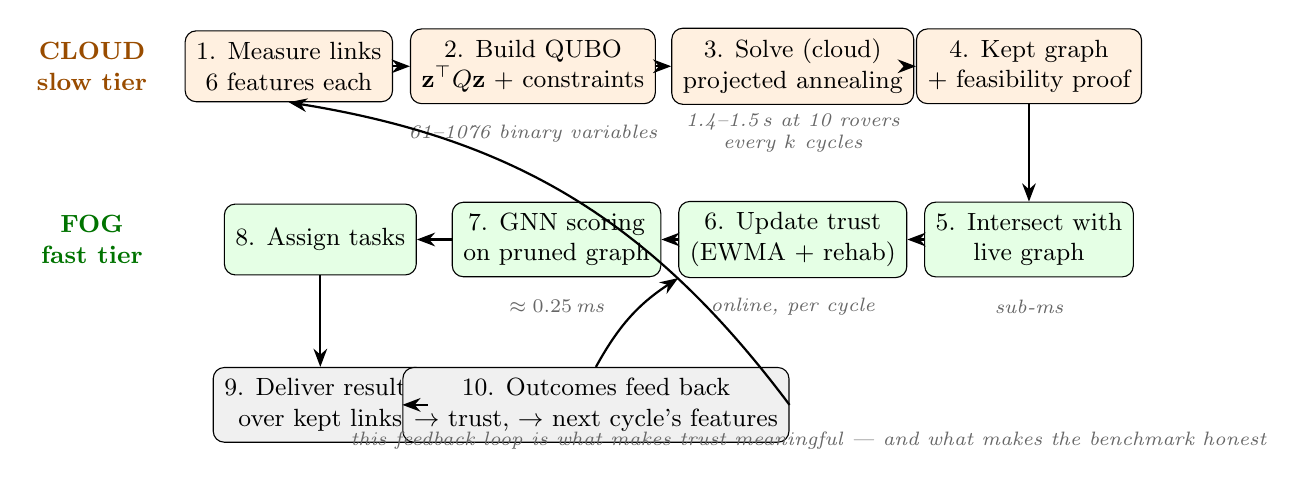
\begin{tikzpicture}[
  box/.style={draw, rounded corners, fill=blue!8, minimum height=9mm,
              align=center, font=\small, inner sep=4pt},
  cloudb/.style={box, fill=orange!12},
  fogb/.style={box, fill=green!10},
  meas/.style={font=\scriptsize\itshape, text=black!60, align=center},
  ar/.style={-Stealth, thick},
  lane/.style={draw, rounded corners, dashed, black!40},
]
  % cloud lane
  \node[cloudb] (feat) at (0,2.2) {1. Measure links\\ 6 features each};
  \node[cloudb] (qubo) at (3.1,2.2) {2. Build QUBO\\ $\mathbf{z}^\top Q \mathbf{z}$
     + constraints};
  \node[cloudb] (solve) at (6.4,2.2) {3. Solve (cloud)\\ projected annealing};
  \node[cloudb] (keep) at (9.4,2.2) {4. Kept graph\\ + feasibility proof};
  \draw[ar] (feat) -- (qubo); \draw[ar] (qubo) -- (solve); \draw[ar] (solve) -- (keep);
  \node[meas] at (3.1,1.35) {61--1076 binary variables};
  \node[meas] at (6.4,1.35) {1.4--1.5\,s at 10 rovers\\ every $k$ cycles};
  % fog lane
  \node[fogb] (intersect) at (9.4,0) {5. Intersect with\\ live graph};
  \node[fogb] (trust) at (6.4,0) {6. Update trust\\ (EWMA + rehab)};
  \node[fogb] (gnn) at (3.4,0) {7. GNN scoring\\ on pruned graph};
  \node[fogb] (assign) at (0.4,0) {8. Assign tasks};
  \draw[ar] (keep) -- (intersect); \draw[ar] (intersect) -- (trust);
  \draw[ar] (trust) -- (gnn); \draw[ar] (gnn) -- (assign);
  \node[meas] at (9.4,-0.85) {sub-ms};
  \node[meas] at (6.4,-0.85) {online, per cycle};
  \node[meas] at (3.4,-0.85) {$\approx 0.25$\,ms};
  % delivery
  \node[box, fill=gray!12] (deliver) at (0.4,-2.1) {9. Deliver results\\ over kept links};
  \node[box, fill=gray!12] (outcome) at (3.9,-2.1) {10. Outcomes feed back\\
      $\rightarrow$ trust, $\rightarrow$ next cycle's features};
  \draw[ar] (assign) -- (deliver); \draw[ar] (deliver) -- (outcome);
  \draw[ar] (outcome.north) to[bend left=14] (trust.south west);
  \draw[ar] (outcome.east) to[bend right=22] (feat.south);
  \node[meas] at (6.6,-2.55) {this feedback loop is what makes trust meaningful --- and what makes the
      benchmark honest};
  % lanes
  \node[font=\small\bfseries, text=orange!60!black, align=center] at (-2.5,2.2) {CLOUD\\ slow tier};
  \node[font=\small\bfseries, text=green!45!black, align=center] at (-2.5,0) {FOG\\ fast tier};
\end{tikzpicture}
\caption{The full loop. The expensive optimization runs rarely, in the
cloud; the cheap decisions run every cycle, on-device. Outcomes feed back
into trust, so both layers learn from the same reality.}
\label{fig:pipeline}
\end{figure}

\begin{card}
\textbf{The one-line version for slides.} \emph{Measure the network
$\rightarrow$ encode ``which links to keep'' as a constrained QUBO
$\rightarrow$ solve it in the cloud $\rightarrow$ run cheap trust-aware GNN
assignment on the surviving graph $\rightarrow$ let outcomes retrain trust.}
\end{card}

Real measured costs per stage (10 rovers, medians over 16 seeds $\times$ 20
cycles):

\begin{table}[h]
\centering
\small
\begin{tabular}{lrl}
\toprule
stage & measured time & note \\
\midrule
pruning decision (threshold) & $0.0065$\,ms & what we're compared against \\
pruning decision (top-$K$) & $0.0075$\,ms & \\
pruning + repair (greedy) & $0.14$--$0.33$\,ms & constraint-aware baselines \\
\key{QUBO solve (projected annealing)} & \key{$1470$\,ms} & cloud tier, amortized \\
GNN inference (pruned graph) & $\approx 0.25$\,ms & fog tier, every cycle \\
\bottomrule
\end{tabular}
\caption{Per-decision wall clock. The QUBO solve is $\approx
5{,}800\times$ the GNN inference it protects --- which is exactly why it
belongs in the cloud tier and why the paper refuses to claim a latency win.}
\end{table}

% ======================================================================
\section{The core idea, on a graph small enough to check by hand}
% ======================================================================

\begin{goldcard}
\textbf{This section is the heart of the story.} Everything the big system
does is already visible in a 5-rover, 7-link example that we can solve
\emph{exactly, by hand, 64 subsets at a time}. Every number below was
computed by the actual code (\code{worked\_example.py}) and cross-checked
three independent ways.
\end{goldcard}

\subsection{The instance}

Five rovers: base $0$, and rovers $\{1,2,3,4\}$. Seven candidate links. The
mission requires rovers $\{2,3,4\}$ to stay connected to the base (rover 1
is a relay, not required). Rules: no rover may use more links than its
degree cap; the kept links' total processing cost must fit in a budget of
12 units; hard link $0\text{--}1$ is always kept (it is rover 1's only
tether).

\begin{table}[h]
\centering
\small
\begin{tabular}{lrrrrrrrr}
\toprule
link & trust & link q. & battery & prox. & fresh. & task & \textbf{utility} & \textbf{cost} \\
\midrule
$0\text{--}1$ (hard) & .90 & .90 & .80 & .70 & .90 & .50 & \textbf{0.810} & 2 \\
$0\text{--}2$ & .90 & .90 & .90 & .90 & .90 & .90 & \textbf{0.900} & 1 \\
$0\text{--}3$ & .40 & .50 & .50 & .40 & .40 & .20 & \textbf{0.405} & 8 \\
$1\text{--}2$ & .80 & .70 & .90 & .60 & .80 & .40 & \textbf{0.705} & 3 \\
$2\text{--}3$ & .70 & .80 & .80 & .70 & .90 & .60 & \textbf{0.750} & 4 \\
$2\text{--}4$ & .85 & .85 & .75 & .80 & .85 & .55 & \textbf{0.790} & 2 \\
$3\text{--}4$ & .60 & .60 & .70 & .50 & .60 & .30 & \textbf{0.555} & 6 \\
\bottomrule
\end{tabular}
\caption{The instance. Utility $=$ weighted sum of the six features
(weights $0.25/0.25/0.10/0.10/0.15/0.15$ --- they sum to 1). Cost is
quantized to integer budget units ($\times 10$). The previous cycle kept
$\{0\text{--}1, 0\text{--}2, 1\text{--}2, 2\text{--}3, 3\text{--}4\}$.}
\end{table}

\subsection{Three ways to be wrong, and one way to be right}

There are $2^6 = 64$ possible keep/drop choices for the six optional links.
The code evaluated \emph{all 64}, checking constraints and computing the
exact QUBO energy of each. Result:

\begin{center}
\begin{tabular}{lrl}
\toprule
outcome & count & meaning \\
\midrule
fully feasible subsets & \key{3} & only 4.7\% of choices are legal \\
connectivity traps & \bad{30} & look great, strand a required rover \\
degree/budget violators & \bad{31} & break the hard rules \\
\bottomrule
\end{tabular}
\end{center}

\begin{figure}[h]
\centering
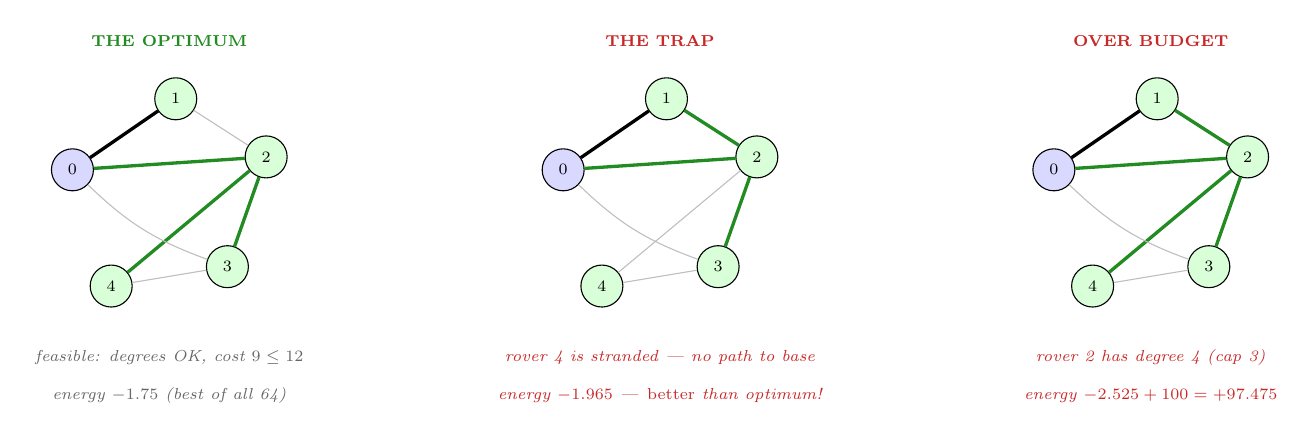
\begin{tikzpicture}[scale=0.82, every node/.style={transform shape},
  rv/.style={draw, circle, fill=green!15, minimum size=6.5mm, font=\scriptsize},
  base/.style={draw, circle, fill=blue!15, minimum size=6.5mm, font=\scriptsize},
  lbl/.style={font=\scriptsize\itshape, text=black!60},
]
  % --- optimum ---
  \begin{scope}[shift={(0,0)}]
    \node[base] (a) at (0,0) {0};
    \node[rv] (b) at (1.6,1.1) {1};
    \node[rv] (c) at (3.0,0.2) {2};
    \node[rv] (d) at (2.4,-1.5) {3};
    \node[rv] (e) at (0.6,-1.8) {4};
    \draw[very thick] (a)--(b); \draw[very thick, goodg] (a)--(c);
    \draw[very thick, goodg] (c)--(d); \draw[very thick, goodg] (c)--(e);
    \draw[black!25] (b)--(c); \draw[black!25] (d)--(e); \draw[black!25] (a) to[bend right=12] (d);
    \node[font=\scriptsize\bfseries, text=goodg] at (1.5,2.0) {THE OPTIMUM};
    \node[lbl] at (1.5,-2.9) {feasible: degrees OK, cost $9\le 12$};
    \node[lbl] at (1.5,-3.5) {energy $-1.75$ (best of all 64)};
  \end{scope}
  % --- trap ---
  \begin{scope}[shift={(7.6,0)}]
    \node[base] (a) at (0,0) {0};
    \node[rv] (b) at (1.6,1.1) {1};
    \node[rv] (c) at (3.0,0.2) {2};
    \node[rv] (d) at (2.4,-1.5) {3};
    \node[rv] (e) at (0.6,-1.8) {4};
    \draw[very thick] (a)--(b); \draw[very thick, goodg] (a)--(c);
    \draw[very thick, goodg] (b)--(c); \draw[very thick, goodg] (c)--(d);
    \draw[black!25] (c)--(e); \draw[black!25] (d)--(e); \draw[black!25] (a) to[bend right=12] (d);
    \node[font=\scriptsize\bfseries, text=badr] at (1.5,2.0) {THE TRAP};
    \node[lbl, text=badr] at (1.5,-2.9) {rover 4 is stranded --- no path to base};
    \node[lbl, text=badr] at (1.5,-3.5) {energy $-1.965$ --- \emph{better} than optimum!};
  \end{scope}
  % --- over budget ---
  \begin{scope}[shift={(15.2,0)}]
    \node[base] (a) at (0,0) {0};
    \node[rv] (b) at (1.6,1.1) {1};
    \node[rv] (c) at (3.0,0.2) {2};
    \node[rv] (d) at (2.4,-1.5) {3};
    \node[rv] (e) at (0.6,-1.8) {4};
    \draw[very thick] (a)--(b); \draw[very thick, goodg] (a)--(c);
    \draw[very thick, goodg] (b)--(c); \draw[very thick, goodg] (c)--(d);
    \draw[very thick, goodg] (c)--(e);
    \draw[black!25] (d)--(e); \draw[black!25] (a) to[bend right=12] (d);
    \node[font=\scriptsize\bfseries, text=badr] at (1.5,2.0) {OVER BUDGET};
    \node[lbl, text=badr] at (1.5,-2.9) {rover 2 has degree 4 (cap 3)};
    \node[lbl, text=badr] at (1.5,-3.5) {energy $-2.525 + 100 = +97.475$};
  \end{scope}
\end{tikzpicture}
\caption{The three most tempting subsets in the example. Left: the true
optimum. Middle: the trap --- a naive ``keep the best-looking links''
pruner takes it, because its energy ($-1.965$) is \emph{lower} than the
optimum's ($-1.75$), and nothing in its field of view says rover 4 is
stranded. Right: the constraint-breaking variant, which the QUBO's penalty
terms price at $+97.475$.}
\label{fig:trap}
\end{figure}

\subsection{The hand-checkable arithmetic}

\begin{card}
\textbf{Optimum} $=\{0\text{--}1,\,0\text{--}2,\,2\text{--}3,\,2\text{--}4\}$:
\begin{itemize}
\item utility of kept optional links: $0.900 + 0.750 + 0.790 = -2.440$
\item sparsity charge: $3 \times 0.08 = +0.240$
\item switching charge vs.\ last cycle: $2\text{--}3$ stays (0),
$2\text{--}4$ switches on ($+0.15$), $1\text{--}2$ switches off ($+0.15$),
$3\text{--}4$ switches off ($+0.15$) $= +0.450$
\item \textbf{energy} $= -2.440 + 0.240 + 0.450 = \key{-1.750}$
\end{itemize}
(The hard link $0\text{--}1$ contributes $-0.810+0.080 = -0.730$ to the
QUBO's \emph{constant} term --- identical for every subset, so it never
changes the ranking.)
Feasibility: cost $2+1+4+2=9\le12$; degrees $3,2,3,2,2$ all within caps;
rovers $\{2,3,4\}$ all reach the base. \checkmark

\textbf{The trap} $=\{0\text{--}1,\,0\text{--}2,\,1\text{--}2,\,2\text{--}3\}$:
utility $0.900+0.705+0.750 = 2.355$; sparsity $3\times0.08=0.240$;
switching: only $3\text{--}4$ turns off ($+0.15$) $\Rightarrow$
$-2.355+0.240+0.150 = \bad{-1.965}$ --- \emph{better} than the optimum, and
degrees ($2,2,3,2$) and cost ($10\le12$) are perfectly legal. Its only flaw
is invisible to a utility-only pruner: \textbf{rover 4 has no path to the
base}. That single number is the entire motivation for constraint-aware
pruning.
\end{card}

\subsection{Three independent solvers, one answer}

\begin{center}
\begin{tabular}{llr}
\toprule
method & what it does & result \\
\midrule
exhaustive enumeration & all 64 subsets, closed-form slacks & \good{$-1.750$} \\
projected annealer (production) & anneals over \emph{feasible} subsets, cold start & \good{$-1.750$} \; \good{exact} \\
MILP / CBC (exact baseline) & linear program with integer links & \good{$-1.750$} \\
\bottomrule
\end{tabular}
\end{center}

And the Q-matrix cross-check: the energy of the optimum's binary vector
computed straight from the exported $61\times61$ matrix $Q$ equals the
enumeration energy to $10^{-9}$. \emph{The encoding is not just plausible;
it is verified.}

\begin{card}
\textbf{Where do 61 variables come from, on a 5-rover graph with 6
decisions?} $6$ edge variables $x_e$ $+$ $13$ degree-slack bits $+$
$28$ flow bits $+$ $14$ flow-capacity bits $= 61$. The extra 55 are the
price of encoding \emph{hard} constraints (degree, budget, and
connectivity-via-single-commodity-flow) inside a purely binary quadratic
form. This is also the seed of the paper's central discovery --- see
Section~\ref{sec:barrier}.
\end{card}

\begin{figure}[h]
\centering
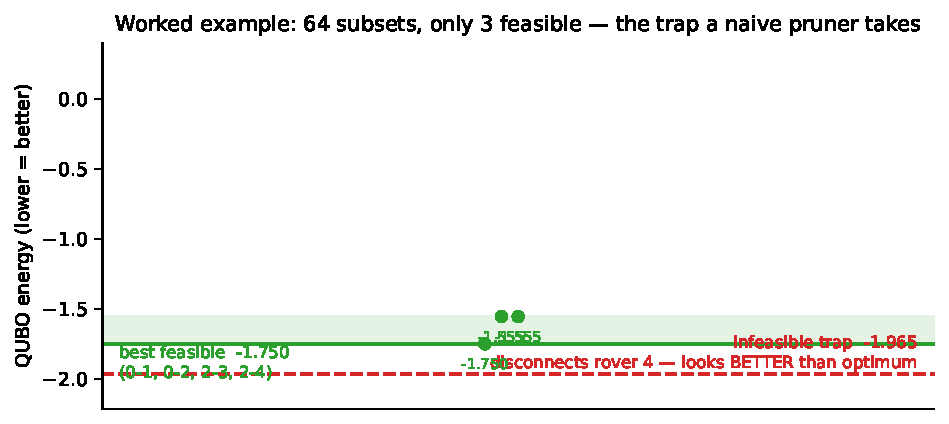
\includegraphics[width=0.86\textwidth]{figs_doc/fig_worked_landscape.pdf}
\caption{The energy landscape of the worked example. Only three subsets are
feasible (green band); the most tempting infeasible one (red) \emph{beats}
the optimum on raw energy. A pruning method without constraint awareness
doesn't just risk being illegal --- it actively prefers the wrong answer.}
\end{figure}

% ======================================================================
\section{The hidden pattern: why generic QUBO solvers fail here}
\label{sec:barrier}
% ======================================================================

\begin{goldcard}
\textbf{The discovery.} On this penalty-encoded landscape, serious
annealing solvers fail not because they are weak but because of the
\emph{shape} of the energy surface. This is the paper's most cited-worthy
finding, and it has a clean one-sentence explanation.
\end{goldcard}

\begin{card}
\textbf{The one-sentence explanation.} From any feasible solution, every
single-bit flip either (a) breaks a constraint and costs at least
$100$ energy points, or (b) stays feasible and changes the score by at
most about $1.2$. The barrier is $\ge 80\times$ taller than the largest
beneficial move --- so at any temperature where good moves are accepted,
bad moves are never accepted, and the sampler \emph{can never leave a
feasible basin}. It is trapped by design.
\end{card}

Empirically, on the actual $Q$ matrices of 25 exactly-verifiable instances:

\begin{center}
\begin{tabular}{lr}
\toprule
solver & exact-solve rate \\
\midrule
simulated quantum annealing (OpenJij) & \bad{48\%} \\
local bit-flip simulated annealing & \bad{56\%} \\
D-Wave \code{neal} & \bad{60\%} \\
tabu search & \bad{64\%} \\
exact linearized solve (CBC) & \good{100\%} \\
projected annealer (ours, engineering note) & \good{100\%} \\
\bottomrule
\end{tabular}
\end{center}

Supporting evidence: random restarts of bit-level annealing returned
\emph{infeasible} states in 19 of 25 instances. The solvers aren't
converging to wrong optima --- they are failing to even find legal ones.

\begin{card}
\textbf{The fix (and its honest caveat).} The production solver,
\emph{projected edge annealing}, stops sampling bit strings and instead
toggles whole edges, projecting every candidate back to full feasibility
(exact slack recomputation + spanning-tree flow) before scoring it.
It solves 100\% of the verifiable instances ($\approx 2.4\times10^4$
energy evaluations, 2.1\,s per solve) and stays within $10^{-3}$ of the
MILP optimum on 20 larger instances (95\% exact). The caveat, which the
paper states plainly: its move set is richer than the bit-samplers', so it
is an \emph{engineering} result, not a scientific one --- and on classical
hardware, CBC solves the same instances exactly in $\approx 15$\,ms, about
$100\times$ faster. \emph{The QUBO's remaining job is to be the input
format for quantum hardware, not to win on a CPU.}
\end{card}

% ======================================================================
\section{How the benchmark works (and how it audited itself)}
% ======================================================================

\subsection{The measurement design}

\begin{card}
\textbf{Simple version.} We run the \emph{identical} simulated world
through six pruning strategies --- same rovers, same drift, same tasks,
seed by seed --- and compare what happens to success, feasibility, and
cost. Because every arm sees the same world, differences are causal, not
luck.
\end{card}

\textbf{Detail.} 6 arms $\times$ 16 seeds $\times$ 20 cycles per
configuration, two budget regimes (nominal fixed $K{=}15$; binding
$K{=}0.75\times$ the full-graph cost), plus three constraint-pressure
sweeps (Section~\ref{sec:pressure}). In total: \key{1{,}152 scenario
cells, $\approx 23{,}000$ simulated rover-cycles}. Paired statistics
(per-seed differences, bootstrap 95\% CIs, sign-flip permutation tests)
because across-seed comparisons understate paired differences.

\textbf{The six arms:}
\begin{enumerate}
\item \textbf{full graph} --- prune nothing (the do-nothing baseline);
\item \textbf{threshold} --- keep every link whose utility beats a cutoff
(constraint-blind);
\item \textbf{top-$K$} --- keep the $K$ best links by utility
(constraint-blind);
\item \textbf{threshold+repair} --- same greedy prune, then the
\emph{same feasibility repair the QUBO gets}: enforce the same degree
caps, the same budget, the same mission connectivity;
\item \textbf{top-$K$+repair} --- same with top-$K$;
\item \textbf{QUBO (ours)} --- the constrained optimization.
\end{enumerate}

Arms 4--5 exist because of a review insight worth repeating: \emph{a
violations table against constraint-blind opponents is a straw man} ---
threshold and top-$K$ have no budget or degree parameters, so of course
they ``violate'' things. The repaired variants are given every constraint
the QUBO has, plus the same repair pass. Any remaining QUBO advantage in
feasibility is then real, not manufactured.

\subsection{The metrics, defined}

\begin{center}
\small
\begin{tabular}{p{3.4cm}p{11.6cm}}
\toprule
metric & definition (as implemented) \\
\midrule
task success & delivered results / assigned tasks, per cycle, averaged over
the episode \\
offload rate & task slots actually assigned / total task slots --- a pruner
that disconnects rovers \emph{strands tasks} and this catches it \\
delivery-failure rate & failed delivery attempts / attempted deliveries ---
catches pruners that keep \emph{weak paths} \\
pruning precision & fraction of kept edges that are delivery-critical \\
pruning recall & fraction of delivery-critical edges that were kept \\
delivery-critical (ground truth) & an edge is critical iff removing it from
the \emph{full} candidate graph strictly reduces the widest-path delivery
bottleneck of any mission-critical node --- recomputed per cycle, a true
counterfactual \\
violations & mean counts per 20-cycle run: per-node degree excess, budget
units overrun, mission nodes unreachable \\
relaxation bookkeeping & every solve logs which constraint level it ran at
(full / no-budget / budget-only / unconstrained / mission-unreachable) ---
the audit trail that caught finding~\ref{find:audit} below \\
\bottomrule
\end{tabular}
\end{center}

\subsection{The audit caught the audit}
\label{find:audit}

\begin{goldcard}
At the paper's \emph{nominal} fixed budget $K{=}15$, the budget is below
the cost of \emph{any} connected subgraph at 10 rovers --- so it can never
be satisfied. The solver's relaxation ladder responded by silently running
\key{319 of 320 cycles without the budget constraint}. The original
comparison table's QUBO row was, unknown to us, effectively unconstrained.
The bookkeeping we built to prove feasibility is what exposed this.
\end{goldcard}

Two consequences, both now in the paper:
\begin{enumerate}
\item All constraint-relevant comparisons were re-run at a
\emph{binding, feasible} budget ($K = 0.75\times$ full-graph cost), where
the QUBO solves in full-constraint mode in \good{320 of 320 cycles} with
\good{zero violations}.
\item The fairness correction cuts both ways: against the constraint-aware
repaired baselines, the QUBO's success deficit shrinks from $-4.8$pp
(vs.\ blind threshold) to $-4.1$pp (vs.\ threshold+repair) --- and at the
nominal (infeasible) budget it was only $-2.1$pp and not significant
($p{=}0.10$). Honest comparisons need honest opponents.
\end{enumerate}

% ======================================================================
\section{Results I: the honest scoreboard}
% ======================================================================

\begin{figure}[h]
\centering
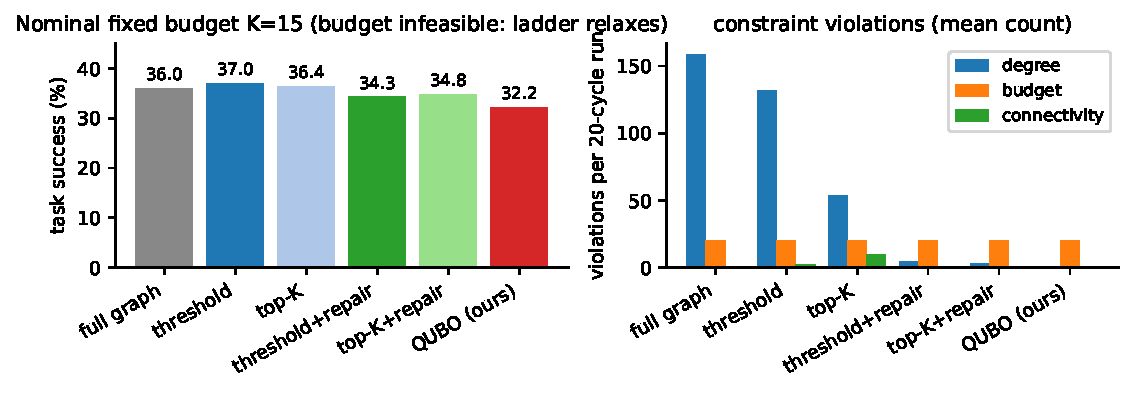
\includegraphics[width=\textwidth]{figs_doc/fig_bench_nominal.pdf}
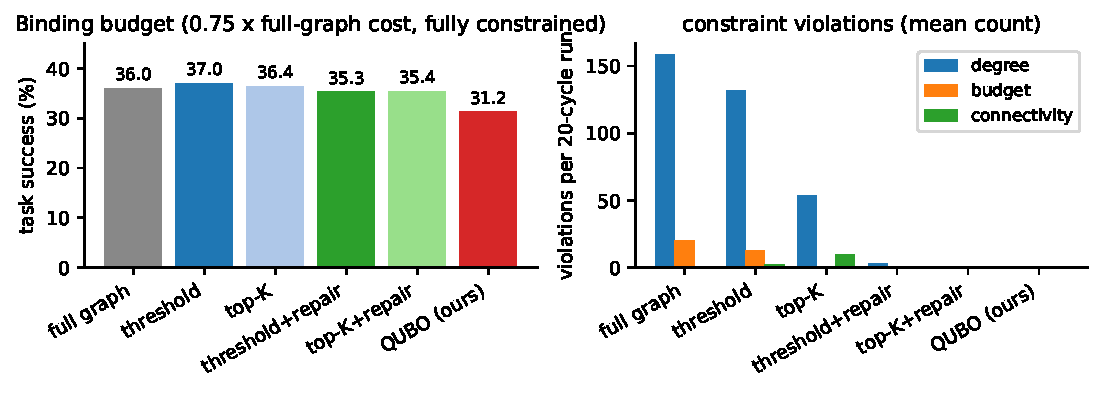
\includegraphics[width=\textwidth]{figs_doc/fig_bench_binding.pdf}
\caption{Top: the nominal-budget benchmark (budget infeasible --- every
arm's budget ``violations'' here reflect the infeasible $K{=}15$, and the
QUBO's ladder relaxes it silently). Bottom: the binding-budget benchmark,
where the QUBO is fully constrained and the guarantees are real. Success
(left) and violations (right), 16 seeds $\times$ 20 cycles.}
\label{fig:bench}
\end{figure}

\begin{table}[h]
\centering
\scriptsize
\begin{tabular}{lrrrrrr}
\toprule
arm (binding budget) & success & offload & del.-fail & solve (ms) & kept & prec.\ / rec.\\
\midrule
full graph & 36.0\% & 100\% & 38.5\% & --- & 100\% & .089 / 1.000 \\
threshold & \textbf{37.0\%} & 95.5\% & \textbf{34.0\%} & $<0.01$ & 84\% & .097 / .931 \\
top-$K$ & 36.4\% & \bad{89.8\%} & \textbf{30.9\%} & $<0.01$ & 50\% & .109 / .562 \\
threshold+repair & 35.3\% & 99.6\% & 38.3\% & 0.33 & 44\% & \textbf{.177} / .817 \\
top-$K$+repair & 35.4\% & 99.7\% & 39.3\% & 0.14 & 42\% & .187 / \textbf{.824} \\
QUBO (ours) & 31.3\% & \good{99.8\%} & \bad{42.7\%} & \bad{1470} & 53\% & .116 / .673 \\
\midrule
\multicolumn{7}{l}{violations per run (degree / budget / connectivity):}\\
full & \multicolumn{2}{r}{158.8 / 20.0 / 0.4} & threshold &
\multicolumn{2}{r}{131.7 / 12.8 / 2.3} & top-$K$: 53.6 / 0 / 10.0 \\
thr+rep & \multicolumn{2}{r}{3.1 / 0.3 / 0.8} & top+rep &
\multicolumn{2}{r}{1.1 / 0 / 0.9} & QUBO: \good{0 / 0 / 0.4} \\
\bottomrule
\end{tabular}
\caption{The full scoreboard at the binding budget. Connectivity misses of
$\approx0.4$ per run appear in \emph{every} arm including the full graph:
those are cycles where the live network itself cannot reach a required
node --- nobody can fix those. Trust metrics: Spearman $0.295$ (QUBO, best)
vs $0.251$--$0.271$; AUC $0.681$ vs $0.624$--$0.683$.}
\label{tab:scoreboard}
\end{table}

\subsection{Reading the scoreboard like a reviewer}

\begin{figure}[h]
\centering
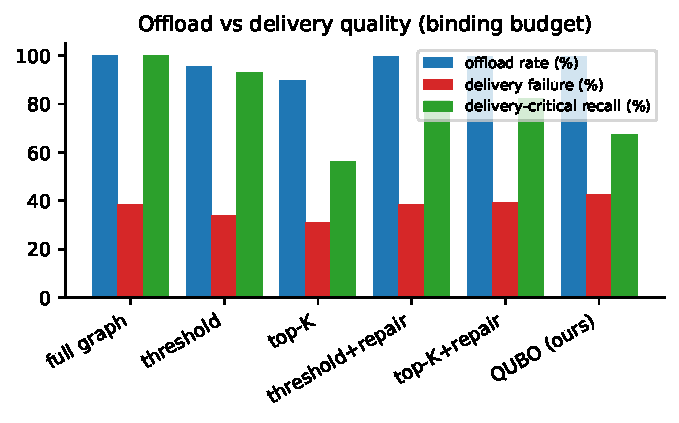
\includegraphics[width=0.62\textwidth]{figs_doc/fig_delivery.pdf}
\caption{The three delivery metrics side by side (binding budget): the
top-$K$ arms trade stranded tasks (offload 89.8\%) for strong paths
(delivery-fail 30.9\%); the QUBO is the mirror image. The repaired
baselines sit in between on both.}
\label{fig:delivery}
\end{figure}

\begin{card}
\textbf{Pattern 1 --- two different failure modes.} Top-$K$ has the
\emph{best} delivery-failure rate (30.9\%) and the \emph{worst} offload
(89.8\%): it prunes so aggressively that it disconnects rovers and
\emph{strands tasks} --- the deliveries it does attempt are over strong
links, but $10.2\%$ of tasks never even launch. The QUBO is the mirror
image: near-perfect offload (99.8\%, nobody stranded) but the \emph{worst}
delivery-failure (42.7\%) --- it keeps everyone connected over paths that
include weak links, because its soft objective misranks delivery-critical
edges (critical recall $0.673$ vs $0.817$--$0.824$ for the repaired
baselines). Same metric table, two completely different diseases.
\end{card}

\begin{card}
\textbf{Pattern 2 --- the guarantee is real and it is the only thing that
is.} At the binding budget the QUBO is the \emph{only} arm with zero
degree and budget violations. The repaired baselines come close (1--3
degree violations per run) but not exact; the blind baselines don't even
try (threshold: 131.7 degree violations, 12.8 budget overruns per run).
\end{card}

\begin{card}
\textbf{Pattern 3 --- the cost of the guarantee, priced.} Paired per-seed
differences at the binding budget: QUBO $-$ threshold+repair $=
-4.1$pp, CI $[-6.4, -1.9]$, $p=0.005$; QUBO $-$ top-$K$+repair $= -4.2$pp,
CI $[-7.0, -1.5]$, $p=0.016$; QUBO $-$ top-$K$ $= -5.1$pp, $p=0.006$. The
guarantee costs about 4 success points at this scale, and the measurement
is tight enough to know it's not noise. \emph{Whether that price is worth
paying is exactly what the next section measures.}
\end{card}

\begin{card}
\textbf{Pattern 4 --- trust quality, with the confound flagged.} The QUBO
arm posts the best Spearman correlation with hidden reliability (0.295 vs
0.251--0.271). But the AUC story is a tie at best (0.681 vs 0.683 for
full/top-$K$), and --- more importantly --- these numbers are measured on
outcomes observed \emph{under each pruner's own policy}. Different pruners
create different observation streams, so the cross-arm trust comparison is
selection-confounded. We say so in the paper rather than harvest the
flattering number.
\end{card}

% ======================================================================
\section{Results II: the constraint-pressure sweep --- does the guarantee ever pay?}
\label{sec:pressure}
% ======================================================================

\begin{goldcard}
\textbf{The question the whole paper hinges on.} ``The QUBO gives
guarantees'' is only a selling point if there is a regime where
\emph{violating} the constraints actually hurts. So we made the constraints
progressively harder and watched for the crossover.
\end{goldcard}

Design: one constraint tightened at a time, ten levels, 16 seeds per cell,
all six arms ---
budget as a fraction $\beta$ of the full-graph cost
($\beta \in \{0.35, 0.5, 0.75, 1.0\}$),
degree cap $D \in \{2,3,4\}$,
mission-critical roster $|R| \in \{3,5,8\}$.

\begin{figure}[h]
\centering
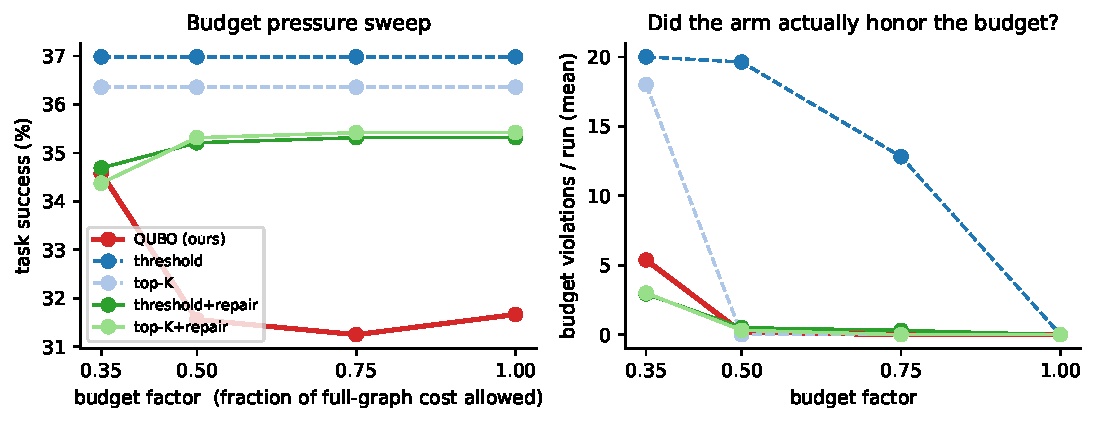
\includegraphics[width=\textwidth]{figs_doc/fig_budget_sweep.pdf}
\caption{Budget pressure. Left: success. Right: budget violations per run
--- the blind threshold pruner violates the budget in 20 of 20 cycles at
$\beta{=}0.35$ and still $12.8$ of 20 at $\beta{=}0.75$, while the QUBO
converges to zero (its small residual at $\beta \le 0.5$ is the ladder
relaxing a genuinely infeasible request, which the bookkeeping counts and
reports).}
\label{fig:budgetsweep}
\end{figure}

\begin{center}
\small
\begin{tabular}{llrrl}
\toprule
constraint & level & QUBO & best repaired & QUBO $-$ best (paired) \\
\midrule
budget $\beta$ & 0.35 & 34.6\% & 34.7\% & $-0.1$pp, $p=1.00$ (tie) \\
budget $\beta$ & 0.50 & 31.6\% & 35.2\% & $-3.7$pp, $p=0.033$ \\
budget $\beta$ & 0.75 & 31.3\% & 35.3\% & $-4.1$pp, $p=0.004$ \\
budget $\beta$ & 1.00 & 31.7\% & 35.3\% & $-3.7$pp, $p=0.020$ \\
degree $D$ & 2 & 30.9\% & 34.3\% & $-3.3$pp, $p=0.15$ \\
degree $D$ & 3 & 32.2\% & 34.3\% & $-2.1$pp, $p=0.10$ \\
degree $D$ & 4 & 33.3\% & 34.8\% & $-0.9$pp, $p=0.52$ \\
roster $|R|$ & 3 & 32.2\% & 34.3\% & $-2.1$pp, $p=0.10$ \\
roster $|R|$ & 5 & 32.4\% & 35.1\% & $-2.7$pp, $p=0.058$ \\
roster $|R|$ & 8 & 34.6\% & 37.8\% & $-3.2$pp, $p=0.020$ \\
\bottomrule
\end{tabular}
\end{center}

(In the degree and roster sweeps the budget stays at the nominal fixed
$K{=}15$, which is infeasible --- that is why every arm shows $\approx 20$
budget violations there; the swept constraint is the one on the x-axis.)

\begin{card}
\textbf{The answer, and it is not the one the pitch predicts.} At extreme
budget pressure ($\beta{=}0.35$) the QUBO \emph{ties} the best repaired
baseline ($-0.1$pp, $p=1.0$) --- there, even the baselines' repair passes
leave residual violations (2.9--3.0 per run) and the gap closes to noise.
Everywhere else the QUBO loses 2--4 points, and the gap \emph{narrows} as
constraints loosen. \bad{There is no crossover.} In this simulator,
honoring constraints exactly never converts into a success advantage ---
even when constraint-blind pruners violate the budget in literally every
cycle. The honest conclusion: \emph{the guarantees are insurance. They are
worth their premium exactly when violations are disqualifying (safety,
contractual, regulatory), not when success is the only currency.} That is
a defensible product claim, and the sweep is what makes it defensible.
\end{card}

\begin{figure}[h]
\centering
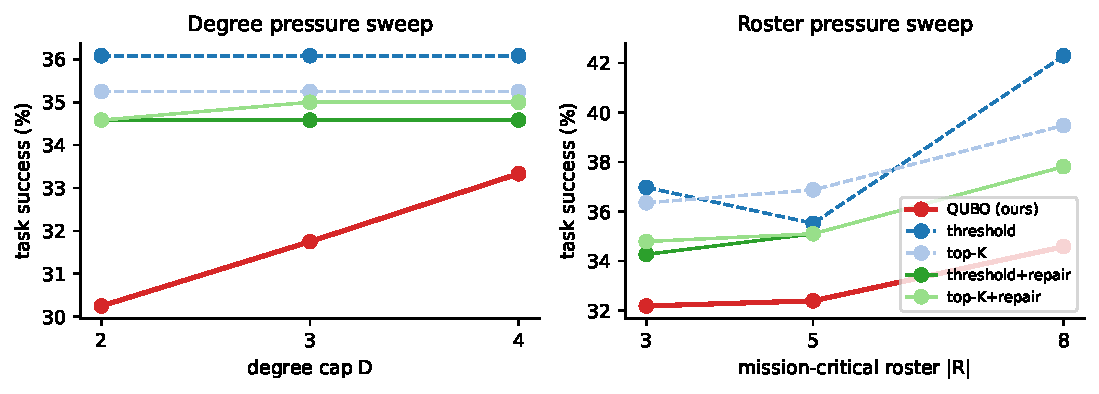
\includegraphics[width=\textwidth]{figs_doc/fig_degree_roster.pdf}
\caption{Degree and roster pressure: same story --- the QUBO's deficit
narrows as the constraint loosens, never reverses.}
\end{figure}

% ======================================================================
\section{Results III: the assignment layer --- where the project genuinely wins}
% ======================================================================

\begin{goldcard}
This is the cleanest positive result in the project, and it is about the
\emph{GNN + trust} layer, not the optimizer.
\end{goldcard}

Four assignment policies, identical worlds, 8 seeds:

\begin{center}
\begin{tabular}{lr}
\toprule
policy & success \\
\midrule
random among eligible rovers & 26.0\% \\
trust-only (bandit-style baseline) & 31.7\% \\
no-graph logistic readout & 38.1\% \\
\good{trust-aware GNN (ours)} & \good{39.8\%} \\
\midrule
GNN $-$ trust-only & $+8.1$pp, CI $[+4.2,+11.7]$, $p=0.016$ \good{significant} \\
GNN $-$ no-graph & $+1.7$pp, CI $[-2.1,+6.9]$, $p=0.736$ \bad{not significant} \\
\bottomrule
\end{tabular}
\end{center}

\begin{card}
\textbf{How to present this without overclaiming.} The GNN beats the
strong simple baseline by 8.1 points with a clean paired statistic ---
that's real and headline-worthy. But the margin over a no-graph readout
(with the same features, no message passing) is $+1.7$pp and statistically
indistinguishable from zero. So the honest attribution is: \emph{most of
the value is the trust model and the path-aware gating; message passing
adds a small, unproven extra at ten-rover density.} The paper says exactly
this. A reviewer is far more likely to believe the $+8.1$ when you volunteer
the $+1.7$.
\end{card}

Two more results in this layer:

\begin{itemize}
\item \textbf{Training the readout on the unbiased exploration subset (78
samples) did not help:} 36.7\% trained vs 32.8\% fixed weights, difference
$-3.9$pp, CI $[-11.7,+11.7]$, $p=0.49$. Reported as the null result it is.
\item \textbf{Fault recovery works:} under a scripted fault (most reliable
rover degraded + packet-loss spike), success returns to its pre-fault
baseline within 3--4 cycles after the fault expires, with the edge
lifecycle (active $\rightarrow$ suspect $\rightarrow$ probation $\rightarrow$
removed) keeping pruned links observable.
\end{itemize}

And the cloud-amortization question --- can we solve rarely instead of
every cycle?

\begin{center}
\begin{tabular}{rrrr}
\toprule
solve interval $k$ & success & solves/cycle & amortized solve \\
\midrule
1 & 30.3\% & 1.00 & 1279\,ms \\
2 & 29.4\% & 0.50 & 618\,ms \\
4 & 26.9\% & 0.25 & 273\,ms \\
8 & 31.9\% & 0.15 & 151\,ms \\
\bottomrule
\end{tabular}
\end{center}

Reusing a two-cycle-old decision costs under one success point while
halving the solve load; beyond that the measurement is dominated by seed
variance (6 seeds), which the paper states rather than drawing a curve
through noise.

% ======================================================================
\section{Results IV: scale --- where the story has to end up}
% ======================================================================

\begin{center}
\begin{tabular}{rrrrrrr}
\toprule
$n$ & $|E|$ & QUBO vars & solve (s) & $E$ projected & $E$ greedy & $E$ MILP \\
\midrule
$10^\dagger$ & 30 & 427 & 12.6 & $-6.39$ & --- & $-6.39$ \\
$20^\dagger$ & 63 & 1076 & 41.4 & $-15.05$ & $-11.76$ & $-15.36$ \\
30 & 95 & 194 & 15.4 & $-21.12$ & $-16.62$ & --- \\
50 & 169 & 328 & 94.5 & $-36.71$ & $-24.30$ & --- \\
\bottomrule
\end{tabular}
\end{center}
($^\dagger$ connectivity enforced only for $n \le 20$ --- stated, not
hidden. At $n{=}20$ the projected annealer is within $2.0\%$ of the exact
MILP optimum; against the repaired greedy it finds $27\%$ better energy at
$n{=}30$ and $51\%$ better at $n{=}50$.)

\begin{card}
\textbf{The scale story in three sentences.} The dense $Q$ matrix grows
quadratically (1{,}076 variables at just 20 rovers), so the formulation as
built tops out at tens of rovers --- a stated limitation, not a surprise.
Solve time grows into the tens of seconds, which is fine only because the
architecture amortizes it in the cloud. And the constrained objective
genuinely shines against greedy at scale ($+51\%$ better energy at
$n{=}50$) --- though at those sizes the wins belong to ``the constrained
objective + feasible-space search,'' not to QUBO \emph{solving} per se,
since CBC is both exact and $\approx100\times$ faster wherever it can
reach.
\end{card}

% ======================================================================
\section{The full scorecard}
% ======================================================================

\begin{center}
\begin{tabular}{p{7.6cm}p{7.6cm}}
\textbf{\good{Where the project wins}} & \textbf{\bad{Where it loses}} \\
\midrule
\good{Formulation correctness:} encoding verified against independent
re-derivation, 64-subset enumeration, and CBC --- three methods, one
answer, $10^{-9}$ agreement. &
\bad{Raw success at 10 rovers:} $-4.1$pp vs repaired baselines
($p{=}0.005$), $-5.1$pp vs blind top-$K$. \\
\good{The penalty-barrier discovery:} a quantified, reproduced explanation
($\ge 80\times$ barrier ratio) of why annealing samplers fail on
penalty-encoded QUBOs (48--64\% exact). &
\bad{Classical speed:} CBC is exact and $\approx 100\times$ faster than
the annealer; the QUBO detour buys nothing on a CPU. \\
\good{Feasibility guarantees:} the only arm with zero violations at every
tested pressure level; blind baselines violate the budget in up to 20/20
cycles. &
\bad{No success crossover:} even at extreme pressure the QUBO only
\emph{ties} ($-0.1$pp, $p{=}1.0$); the guarantee never converts into
success in this simulator. \\
\good{Assignment layer:} $+8.1$pp over trust-only ($p{=}0.016$), $+13.8$pp
over random, with paired statistics. &
\bad{Message passing unproven:} $+1.7$pp over a no-graph readout,
$p{=}0.736$. \\
\good{Offload guarantee:} 99.8\% of tasks actually assigned (top-$K$:
89.8\% --- it strands tasks). &
\bad{Delivery quality:} worst delivery-failure rate (42.7\%) and lowest
critical recall (0.67) --- the soft objective misranks delivery-critical
edges. \\
\good{Audit culture:} the harness caught its own infeasible budget
(319/320 relaxed cycles) and forced an honest re-run. &
\bad{Small-scale economics:} a 1.47\,s solve protecting 0.25\,ms of
inference ($\approx 5{,}800\times$) only makes sense amortized in the
cloud, or at scale. \\
\end{tabular}
\end{center}

% ======================================================================
\section{Reproducibility --- how to show any of this live}
% ======================================================================

\begin{card}
\begin{tabular}{ll}
\toprule
to demonstrate & run \\
\midrule
the worked example (all 64 subsets, 3-way agreement) &
\code{python worked\_example.py} \\
the pruner benchmark (both budgets, resumable) &
\code{python benchmark\_full.py [start] [end] [budget\_factor]} \\
the constraint-pressure sweeps (resumable) &
\code{python constraint\_pressure.py budget|degree|roster} \\
extract every quoted number & \code{python analyze\_results.py} \\
regenerate every figure in this document & \code{python make\_figures.py} \\
the 486-check regression suite & \code{python battle\_test.py} \\
\bottomrule
\end{tabular}
\end{card}

Every number in this document traces to a JSONL artifact or the worked
example; \code{make\_figures.py} writes \code{doc\_data.json} containing
each quoted aggregate so text and figures cannot drift apart.

% ======================================================================
\section{The one-slide cheat sheet}
% ======================================================================

\begin{goldcard}
\textbf{Ten numbers to memorize for the talk:}
\begin{enumerate}
\item 64 subsets $\rightarrow$ only \textbf{3 feasible}; the best-looking
illegal one scores \textbf{$-1.965$} vs the true optimum \textbf{$-1.75$}
--- constraints change the answer, not just check it.
\item The QUBO for that toy has \textbf{61 variables} (6 edges + 55
constraint bookkeeping) --- constraints are expensive to encode, which is
the seed of the barrier problem.
\item Solver audit: annealers solve \textbf{48--64\%} of verifiable
instances; barrier ratio $\ge \textbf{80}\times$; projected annealer and
CBC: \textbf{100\%}.
\item CBC: exact in \textbf{$\approx15$\,ms}; annealer 2.1\,s --- the QUBO's
job is the hardware interface, not classical speed.
\item Production solve: \textbf{1.47\,s} at 10 rovers vs threshold's
\textbf{0.007\,ms}; GNN inference \textbf{0.25\,ms} ($\approx5{,}800\times$
ratio) $\Rightarrow$ cloud amortization is mandatory ($k{=}8$: 151\,ms,
31.9\%).
\item Success: QUBO \textbf{31.3\%} vs threshold \textbf{37.0\%} at 10
rovers ($-4.1$pp vs repaired baselines, $p{=}0.005$) --- the honest price
of guarantees at small scale.
\item The guarantee itself: \textbf{zero} degree/budget violations at the
binding budget; blind threshold violates the budget \textbf{20/20 cycles}
at extreme pressure.
\item Constraint-pressure sweep: \textbf{no crossover} --- tie at extreme
pressure ($-0.1$pp, $p{=}1.0$), 2--4pp deficit elsewhere. Guarantees are
insurance.
\item Offload vs delivery: QUBO offloads \textbf{99.8\%} (top-$K$ 89.8\%)
but has the worst delivery-failure (\textbf{42.7\%} vs 30.9\%) --- two
different failure modes, both measurable.
\item Assignment layer: \textbf{$+8.1$pp} over trust-only ($p{=}0.016$) ---
the project's cleanest win; message passing itself: $+1.7$pp ($p{=}0.74$),
honestly reported as unproven.
\end{enumerate}
\end{goldcard}

\begin{center}
\begin{tabular}{p{0.9cm}p{5.6cm}p{8.2cm}}
\toprule
slide & claim & evidence to show \\
\midrule
1 & the problem & the dynamic-graph picture (Fig.~1) \\
2 & the pipeline & Fig.~\ref{fig:pipeline} with timings \\
3 & pruning is constrained optimization & worked example + trap figure
(Fig.~\ref{fig:trap}) \\
4 & the encoding is verified & 3-way agreement, $10^{-9}$ \\
5 & generic QUBO solvers fail & audit bar chart, barrier explanation \\
6 & our solver + honest CBC comparison & 100\% exact, 2.1\,s vs 15\,ms \\
7 & the benchmark design & 6 arms, paired stats, metric definitions \\
8 & the honest scoreboard & Fig.~\ref{fig:bench}, Table~\ref{tab:scoreboard} \\
9 & does the guarantee ever pay? & budget-sweep figure, ``no crossover'' \\
10 & what actually wins & $+8.1$pp assignment, offload guarantee, audit \\
\bottomrule
\end{tabular}
\end{center}

\end{document}
